\section{Main Window}
\label{sec:ui_main_window} 

When the application is started for the first time, the main window is shown as follows. 

\begin{figure}[H]
  %\hspace*{-2.5cm}
  \center
    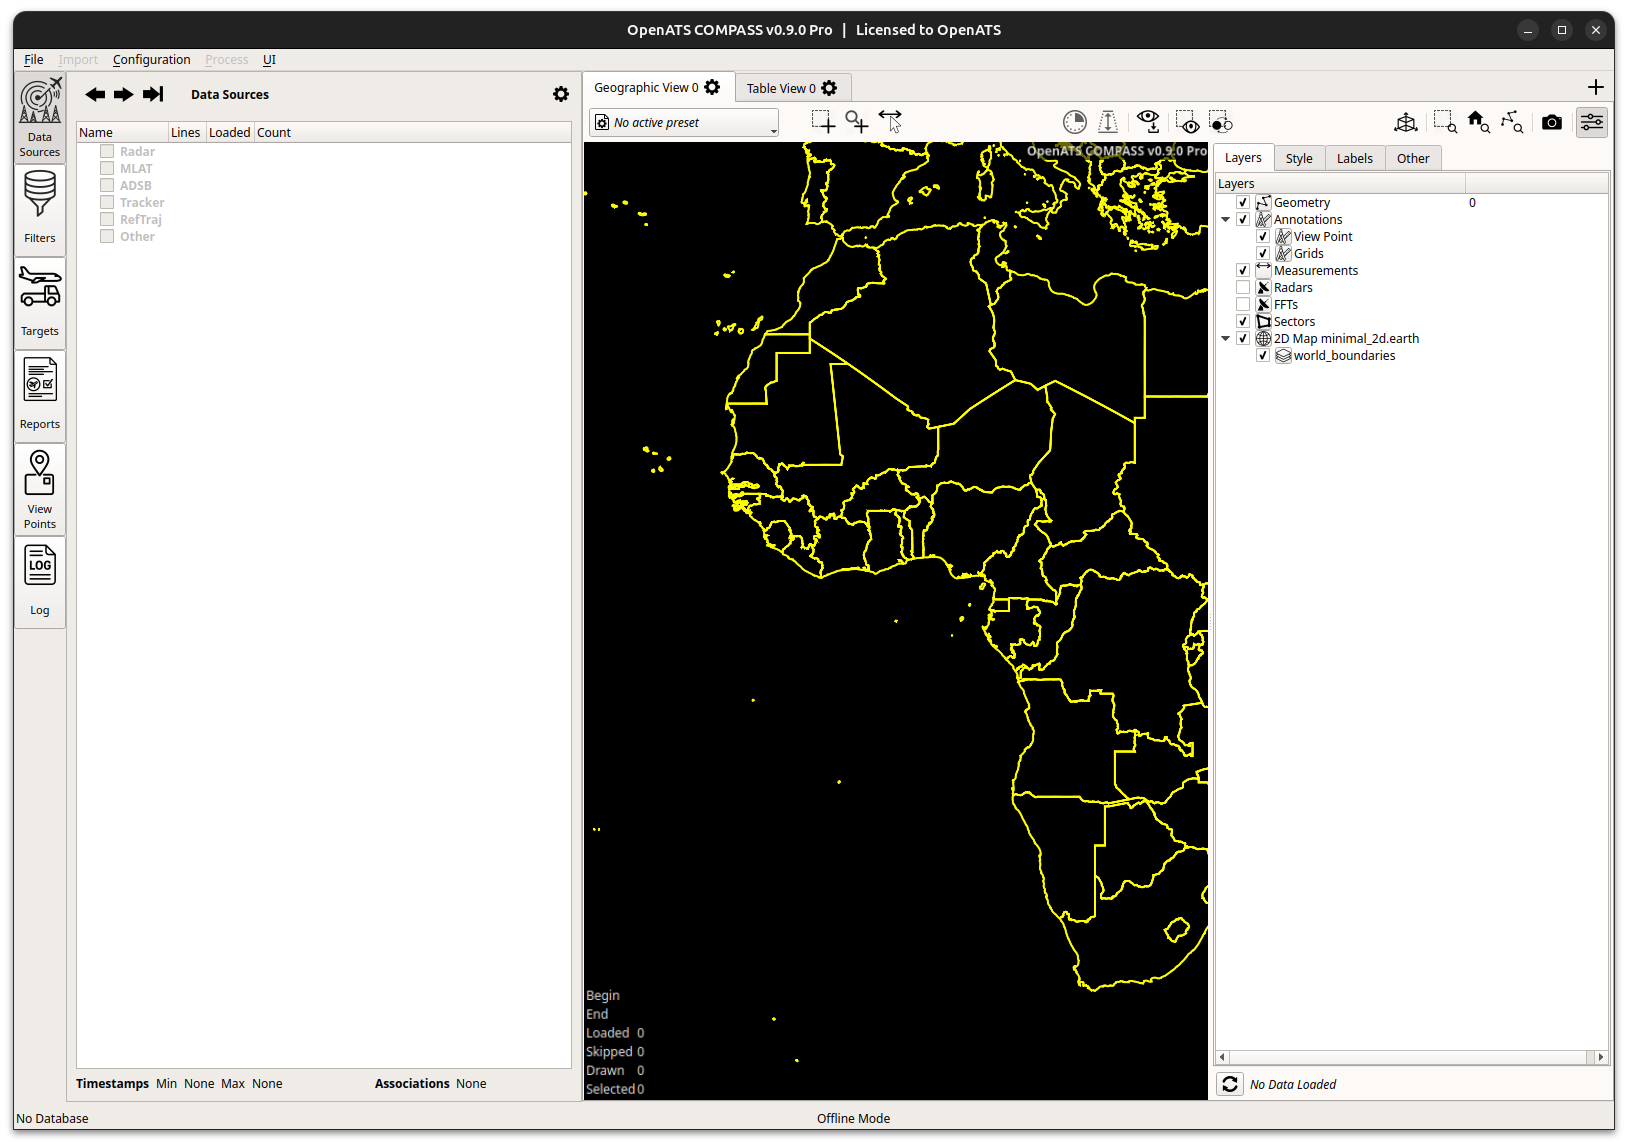
\includegraphics[width=15cm]{figures/main_window.png}
  \caption{Main Window}
\end{figure}

In the simplest use case, the \nameref{sec:ui_main_menu_bar} allows to open or create a database and import data.
After this step, data of interest can be chosen using tools located in the so-called \nameref{sec:ui_flight_deck}, 
and loaded from the database using the 'Load' button of the \nameref{sec:ui_main_status_bar}. 
The loaded data is then shown in Views located either in the \nameref{sec:ui_main_view_bar}, or in other windows. \\

The values set in the 'Data Sources' and 'Filter' tools of the Flight Deck define the dataset loaded from the database into memory (RAM). 
Only the data required by the application is loaded into memory. \\

Only one dataset can exist at a time. At the beginning of a loading process, the old dataset is cleared, and a new one is filled sequentially from the database. 
This single dataset is then distributed to all existing views. \\

When new Views are added, or Views require additional data, a manual reload has to be performed by the user. \\

To close the application either the 'File' menu or the close button in the main window's decoration bar can be used. \\

Please \textbf{note} that using the close button in windows other than the main window only closes the respective window and its Views, but not the application.

Please \textbf{note} that depending on the application status some parts of the UI are inaccessible, e.g. are only available when a database was opened.

\subsection{Main Menubar}
\label{sec:ui_main_menu_bar}

At the top of the Main Window exists the Main Menubar, which contains the Main Menu and allows access to the following sub-menus: 

\begin{itemize}
 \item \nameref{sec:ui_overview_file_menu}: Open/close a database, quit application
 \item \nameref{sec:ui_overview_import_menu}: Import ASTERIX, NMEA data
 \item \nameref{sec:ui_overview_config_menu}: Configure data sources, sectors, manage licenses
 \item \nameref{sec:ui_overview_process_menu}: Various processing tasks for imported data
 \item \nameref{sec:ui_overview_ui_menu}: Reset Views
\end{itemize} 
\  \\

A common workflow is to open or create a database using the 'File' menu. If new data is to be imported, this can be done using the 'Import' menu. 
After all data was imported, the 'Process' menu can be used to post-process the data (if desired). \\

For a more detailed description of the Main Menu's contents refer to section \nameref{sec:main_menu}.

\subsection{Flight Deck} 
\label{sec:ui_flight_deck}

\begin{figure}[H]
  \hspace*{-2.5cm}
  \center
  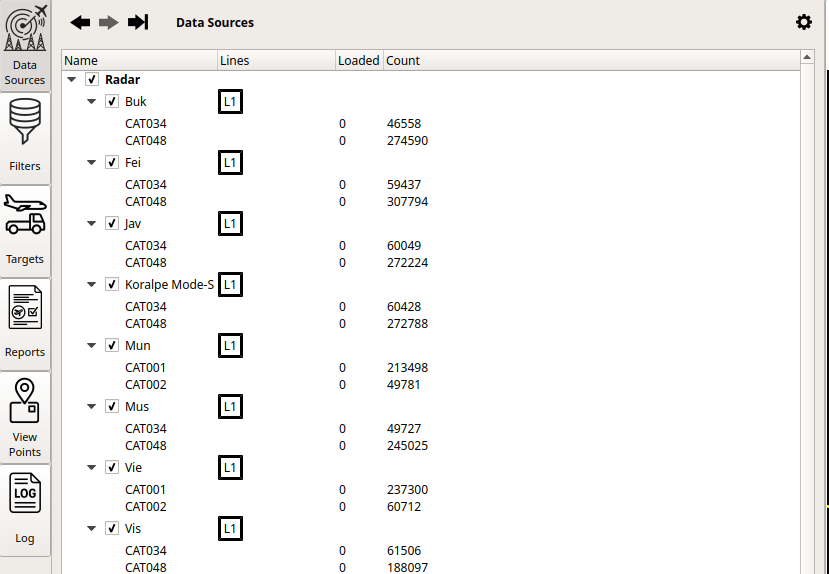
\includegraphics[width=12cm]{figures/ui_flight_deck.png}
  \caption{Opened Flight Deck}
\end{figure}

The Flight Deck is a special tool bar located on the left side of the main window, and allows for quick access to 
frequently used functionality. It can be quickly expanded and collapsed, and its tools can be viewed alongside a View,
making working in a single monitor setup more comfortable. \\

The following tools exist in the Flight Deck:

\begin{table}[H]
  \center
  \begin{tabular}{ | l | l | l | }
    \hline
    \textbf{Tool} & \textbf{Hotkey} & \textbf{Description} \\ \hline
    \nameref{sec:data_sources} & 1 & Select which data sources and lines should be loaded \\ \hline
    \nameref{sec:filters} & 2 & Filter which data should be loaded \\ \hline
    \nameref{sec:targets} & 3 & Allows inspection of unique targets after reference reconstruction \\ \hline
    \nameref{sec:reports} & 4 & Allows inspection of previously generated Reports (e.g. Evaluation Reports) \\ \hline
    \nameref{sec:view_points} & 5 & Show/edit specific cases saved as View Points \\ \hline
    \nameref{sec:task_log} & 6 & Persistent event log, showing important events occurring during COMPASS usage \\ \hline
  \end{tabular}
  \caption{Flight Deck: Available tools}
  \label{table:ui_flight_deck_tools}
\end{table}

% \begin{itemize}
%  \item \nameref{sec:ui_data_sources}: Select which data sources and lines should be loaded
%  \item \nameref{sec:ui_filters}: Filter which data should be loaded
%  \item \nameref{sec:ui_targets}: Allows inspection of unique targets after reference reconstruction
%  \item \nameref{sec:reports}: Allows inspection of previously generated Reports (e.g. Evaluation Reports) %adapting/defining requirement-based standards and compliance assessment of said standards
%  \item \nameref{sec:view_points}: Show/edit specific cases saved as View Points
%  \item \nameref{sec:log}: Persistent event log, showing important events occurring during COMPASS usage (information, warnings, errors)
% \end{itemize}
% \  \\

The individual tools will be described in more detail in Chapter \nameref{chap:flight_deck}. \\

A tool can be selected by clicking its respective icon. This will also show the Flight Deck again if it was previously closed.
Clicking the icon of a selected tool again will close the Flight Deck. Switching between tools can also be achieved by pressing
the number keys on the keyboard. Pressing the respective number key will show the tool (and possibly show the Flight Deck again),
pressing it again will hide the Flight Deck. Table \ref{table:ui_flight_deck_tools} lists the assigned number hotkeys. \\

When selecting a tool, the tools content will be shown with a decoration bar on top. The bar will show the selected tool's name 
and various action buttons for configuring the tool.

\begin{table}[H]
  \center
  \begin{tabular}{ | l | l | l | l |}
    \hline
    \textbf{Icon} & \textbf{Shortcut} &\textbf{Text} & \textbf{Description} \\ \hline
    \includegraphics[width=0.5cm,frame]{../../data/icons/arrow_to_left.png} & - & Decrease Width & Decrease Flight Deck width for the selected tool \\ \hline
    \includegraphics[width=0.5cm,frame]{../../data/icons/arrow_to_right.png} & + & Increase Width & Increase Flight Deck width for the selected tool \\ \hline
    
\includegraphics[width=0.5cm,frame]{../../data/icons/fd_expand.png}/
\includegraphics[width=0.5cm,frame]{../../data/icons/fd_shrink.png} & \# & Expand/Collapse Flight Deck & Enable/Disable Expansion Mode \\ \hline
    \includegraphics[width=0.5cm,frame]{../../data/icons/edit.png} & & & Open the selected tool's configuration menu \\ \hline
  \end{tabular}
  \caption{Toolbar: Available actions}
\end{table}

\paragraph{Expansion Mode} Expansion Mode can be enabled by pressing the 
\includegraphics[width=0.5cm,frame]{../../data/icons/fd_expand.png} 
button or the \# key. In this mode the Flight Deck will overlap all opened Views and use almost the whole Main Window's width.
This mode can be used for a more detailed inspection of a tool's contents (e.g. tables). Pressing the 

\includegraphics[width=0.5cm,frame]{../../data/icons/fd_shrink.png} button or again the \# key will collapse the Flight Deck
back to the selected tool's width. \\

Please \textbf{note} that expanding the Flight Deck will deactivate interaction with the Main Window's Views until the Flight Deck
is collapsed again.

\paragraph{Tool Configuration Menu} Pressing the \includegraphics[width=0.5cm,frame]{../../data/icons/edit.png} button will 
open a menu with tool-specific configuration options. Common to all menus is the 'Screen Ratio' option, where the width the 
Flight Deck occupies in the Main Window can be set by hand for the selected tool, alternatively to pressing 
\includegraphics[width=0.5cm,frame]{../../data/icons/arrow_to_left.png}/\includegraphics[width=0.5cm,frame]{../../data/icons/arrow_to_right.png}.

\begin{figure}[H]
  \hspace*{-2.5cm}
  \center
  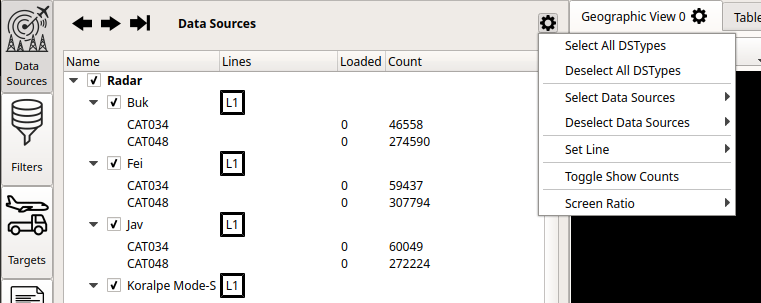
\includegraphics[width=12cm]{figures/ui_flight_deck_config.png}
  \caption{Flight Deck: Tool configuration menu}
\end{figure}

\subsection{Main Viewbar}
\label{sec:ui_main_view_bar}

The Main Viewbar is a tab bar containing the Views added to the Main Window. \\

To add additional views, the \includegraphics[width=0.5cm,frame]{../../data/icons/crosshair_fat.png} button can be used. 
Views can be added either to the window in which the button was clicked ('Add Here') or in a new window ('Add In New Window'). \\

A single View can be removed by clicking the \includegraphics[width=0.5cm,frame]{../../data/icons/edit.png} button in its tab (next to the Views name) and selecting 'Close'. \\

\textbf{Note} that this also applies to the View tab bars of other COMPASS windows. \\

See section \nameref{sec:ui_views} for more details about Views.

\subsection{Main Statusbar}
\label{sec:ui_main_status_bar}

The Main Statusbar at the bottom shows general information and contains the 'Load' button used to trigger a loading process (only visible when a database was opened). \\

The following information is shown:

\begin{itemize}
 \item Database indicator: Shows 'No Database' or currently opened database file name
 \item Application mode: 'Offline' or 'Live'
\end{itemize}
\  \\
